\chapter{Analisi di Stabilità e Linearizzazione}
l'analisi di stabilità e la sintesi dei sistemi di controllo di volo (FCS) richiedono un modello lineare tempo-invariante (LTI). In questo capitolo si descrive la procedura matematica, validata tramite gli script MATLAB, per estrarre il modello nello \textit{Spazio degli Stati} e valutarne la stabilità intrinseca intorno a un punto di \texttt{Trim}. Sarà proprio su questo punto operativo che verranno sintetizzati i controllori avanzati LQR (Cap.\ref{cap:lqr}) e MPC (Cap.\ref{cap:mpc}), valutandone il Control-Invariant-Set e il dominio di attrazione.

\section{Definizione dei punti di equilibrio}
Il volo in condizione di \textit{Trim} è definito come uno stato in cui il velivolo mantiene una traiettoria costante senza accelerazioni nette ($\dot{\mathbf{V}} = \mathbf{0}$, $\dot{\boldsymbol{\omega}} = \mathbf{0}$). Matematicamente, dato il sistema $\dot{\mathbf{X}} = \mathbf{f}(\mathbf{X}, \mathbf{U})$, si ricerca un punto operativo (Operating Point, \texttt{op}) identificato dalla coppia $(\mathbf{X}^*, \mathbf{U}^*)$ tale per cui il campo vettoriale delle derivate si annulli.

\subsection{L'Oggetto opspec (Operating Point Specification)}
Prima di avviare l'algoritmo di ricerca, il software deve conoscere i vincoli del problema. L'oggetto \textbf{\texttt{opspec}} funge da  specifica per la ricerca del punto operativo, istruendo il solutore su quali variabili sono fisse e quali sono libere di variare:
\begin{itemize}
    \item \textbf{Stati Fissati (\texttt{Known = true}):} Si impone una condizione di volo specifica, ad esempio una velocità costante $V_t = 91.44$ m/s e quota fissa.
    \item \textbf{Derivate Nulle (\texttt{SteadyState = true}):} Si impone che le accelerazioni siano zero. Fanno eccezione le coordinate di posizione Nord ed Est (\texttt{SteadyState = false}), poiché l'aereo si sposta nello spazio, ma questo non altera l'equilibrio delle forze aerodinamiche.
    \item \textbf{Limiti (\texttt{Min / Max}):} Si impongono vincoli fisici, come la saturazione della spinta ($T \in [1000, 19000]$ lbf) o il finecorsa meccanico dell'equilibratore ($\pm 25^\circ$). Tali limiti fisici costituiranno i vincoli per la definizione dell'Invariant Set nella sintesi del controllo MPC, come verrà approfondito nel Capitolo \ref{cap:mpc}.
\end{itemize}

\subsection{Generazione di op e opreport}
Completato il setup, la funzione MATLAB \texttt{findop} viene richiamata per calcolare il punto di equilibrio. Data la forte non linearità del modello aerodinamico dell'F-16 e i stringenti vincoli fisici imposti tramite l'oggetto \texttt{opspec}, i tradizionali algoritmi di ottimizzazione locale (come il \textbf{Gradiant-Descent} e \textbf{Active-Set}), tendono spesso a bloccarsi in minimi locali o a fallire la convergenza, tali algoritmi, testati in ambiente MATLAB, hanno restituito punti operativi sub-ottimi che non soddisfano le rigorose specifiche imposte nell'oggetto opspec. Per superare questa criticità e ottenere un punto operativo fisicamente accettabile che rispettasse rigorosamente le specifiche, si è reso necessario l'utilizzo di un algoritmo di ottimizzazione globale ed euristico chiamato (\textbf{Particle Swarm Optimization})\cite{Particle_Swarm_Optimization}. \begin{figure}[H]
	\centering
	% Sostituisci 'punto_operativo.png' con il nome esatto del tuo screenshot caricato su Overleaf
	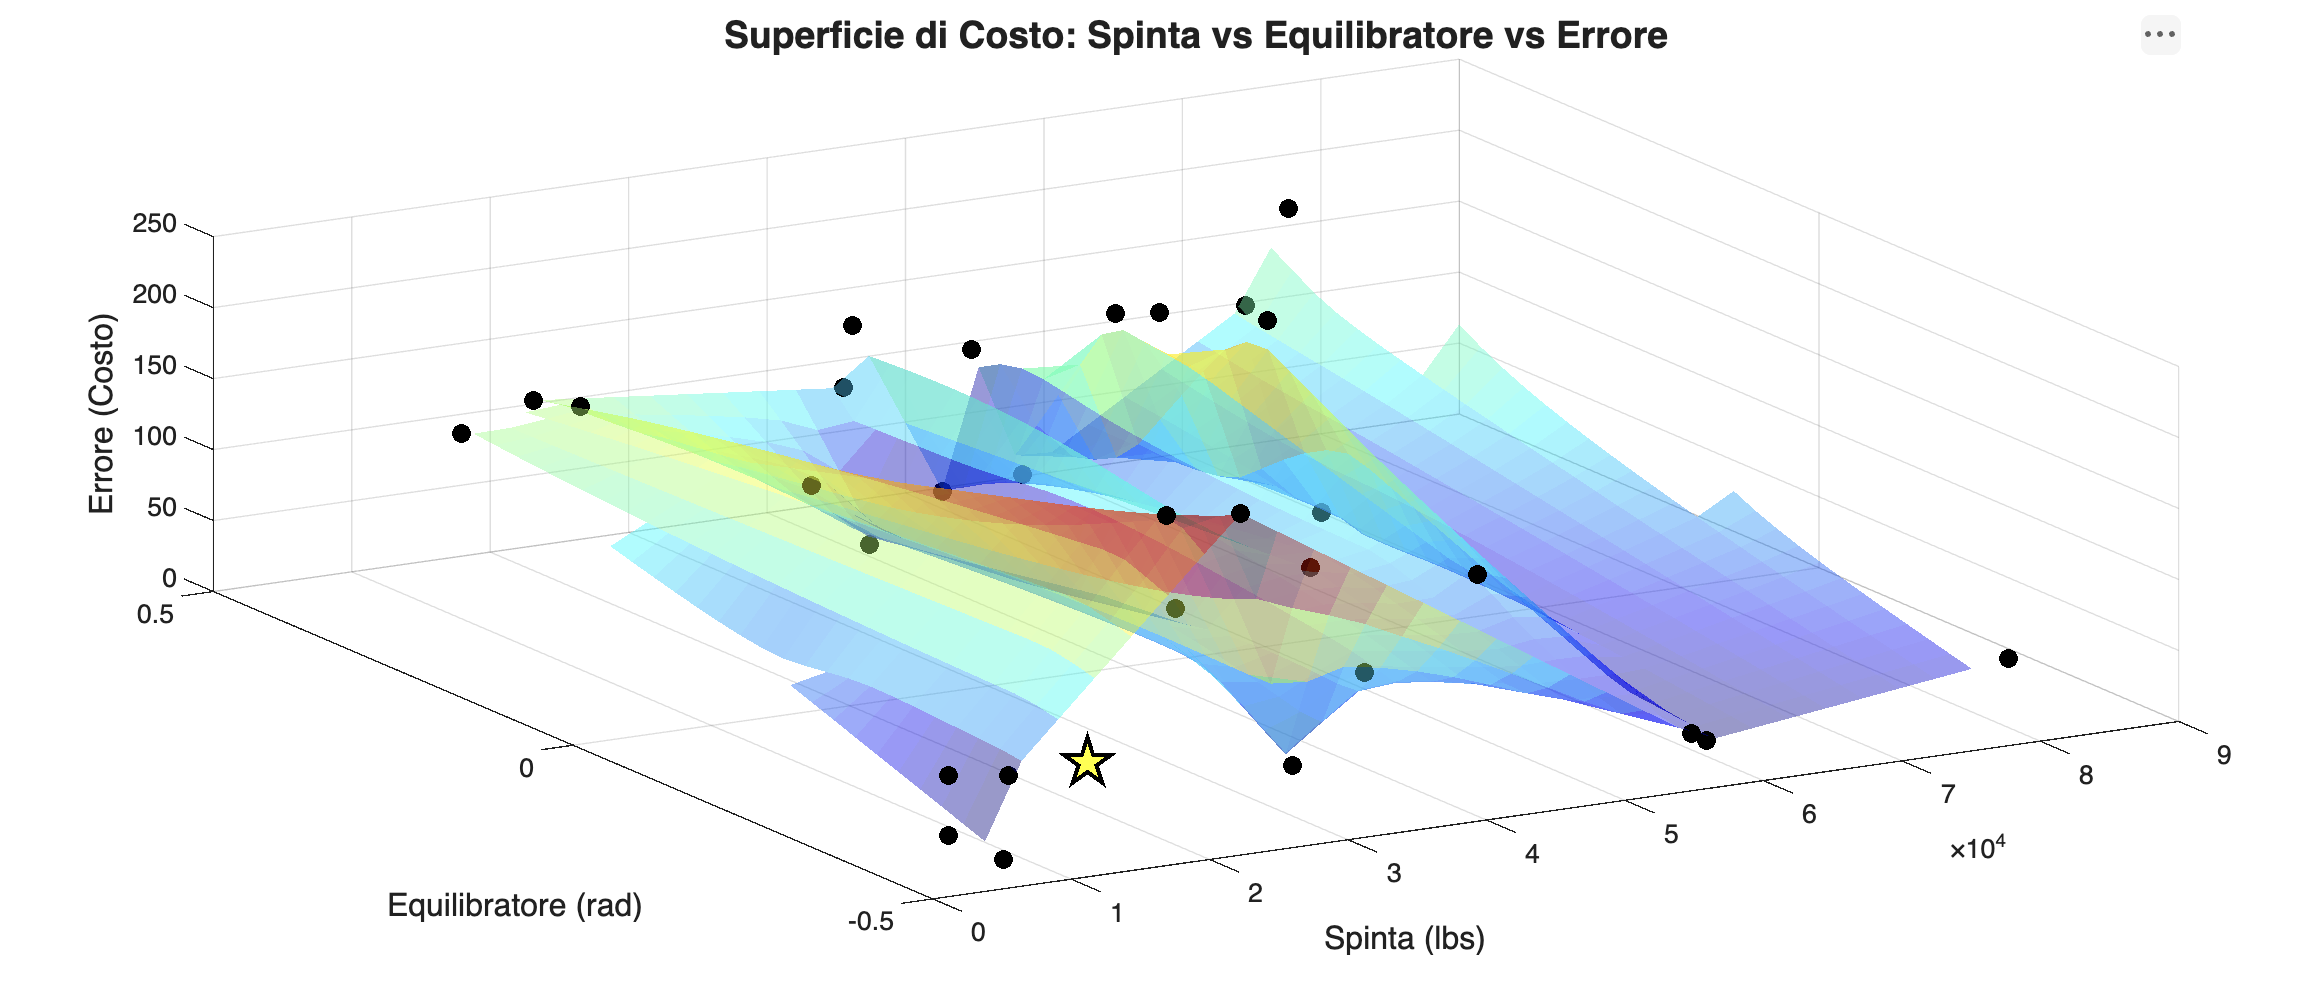
\includegraphics[width=1\textwidth]{Foto/AlgoritmoPSO_Inizio.png}
	\caption{Inizio della ricerca dell'algortimo PSO}
	\label{fig:PSO}
\end{figure}
\begin{figure}[h!]
	\centering
	% Sostituisci 'punto_operativo.png' con il nome esatto del tuo screenshot caricato su Overleaf
	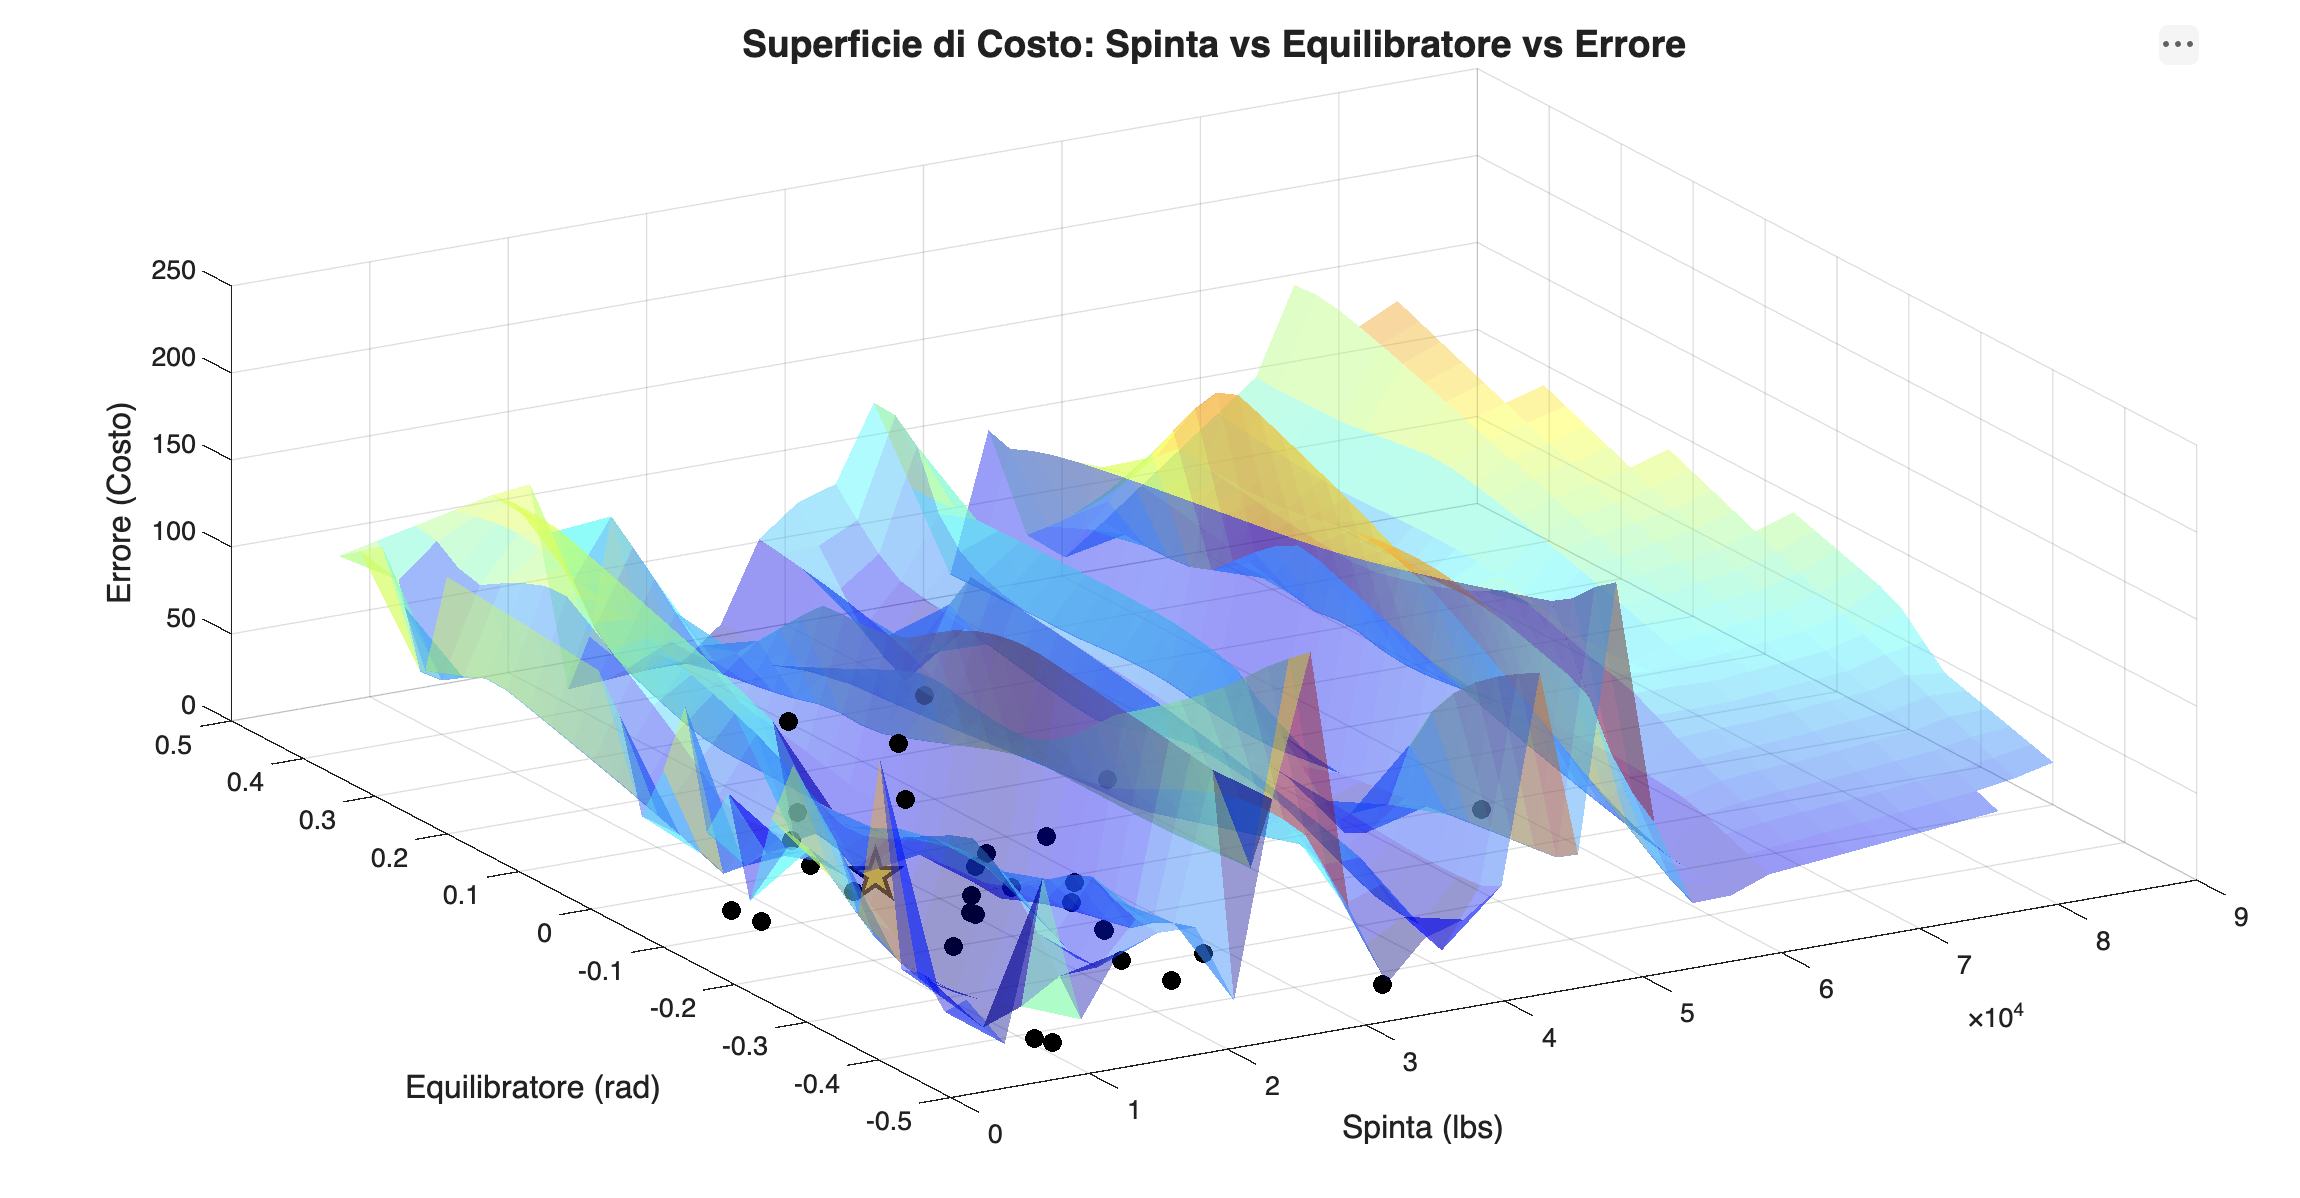
\includegraphics[width=1\textwidth]{Foto/AlgortimoPSO_Mezzo.png}
	\caption{Algortimo PSO a metà del suo funzionamento}
	\label{fig:PSO_mezzo}
\end{figure}


\begin{figure}[H]
	\centering
	 	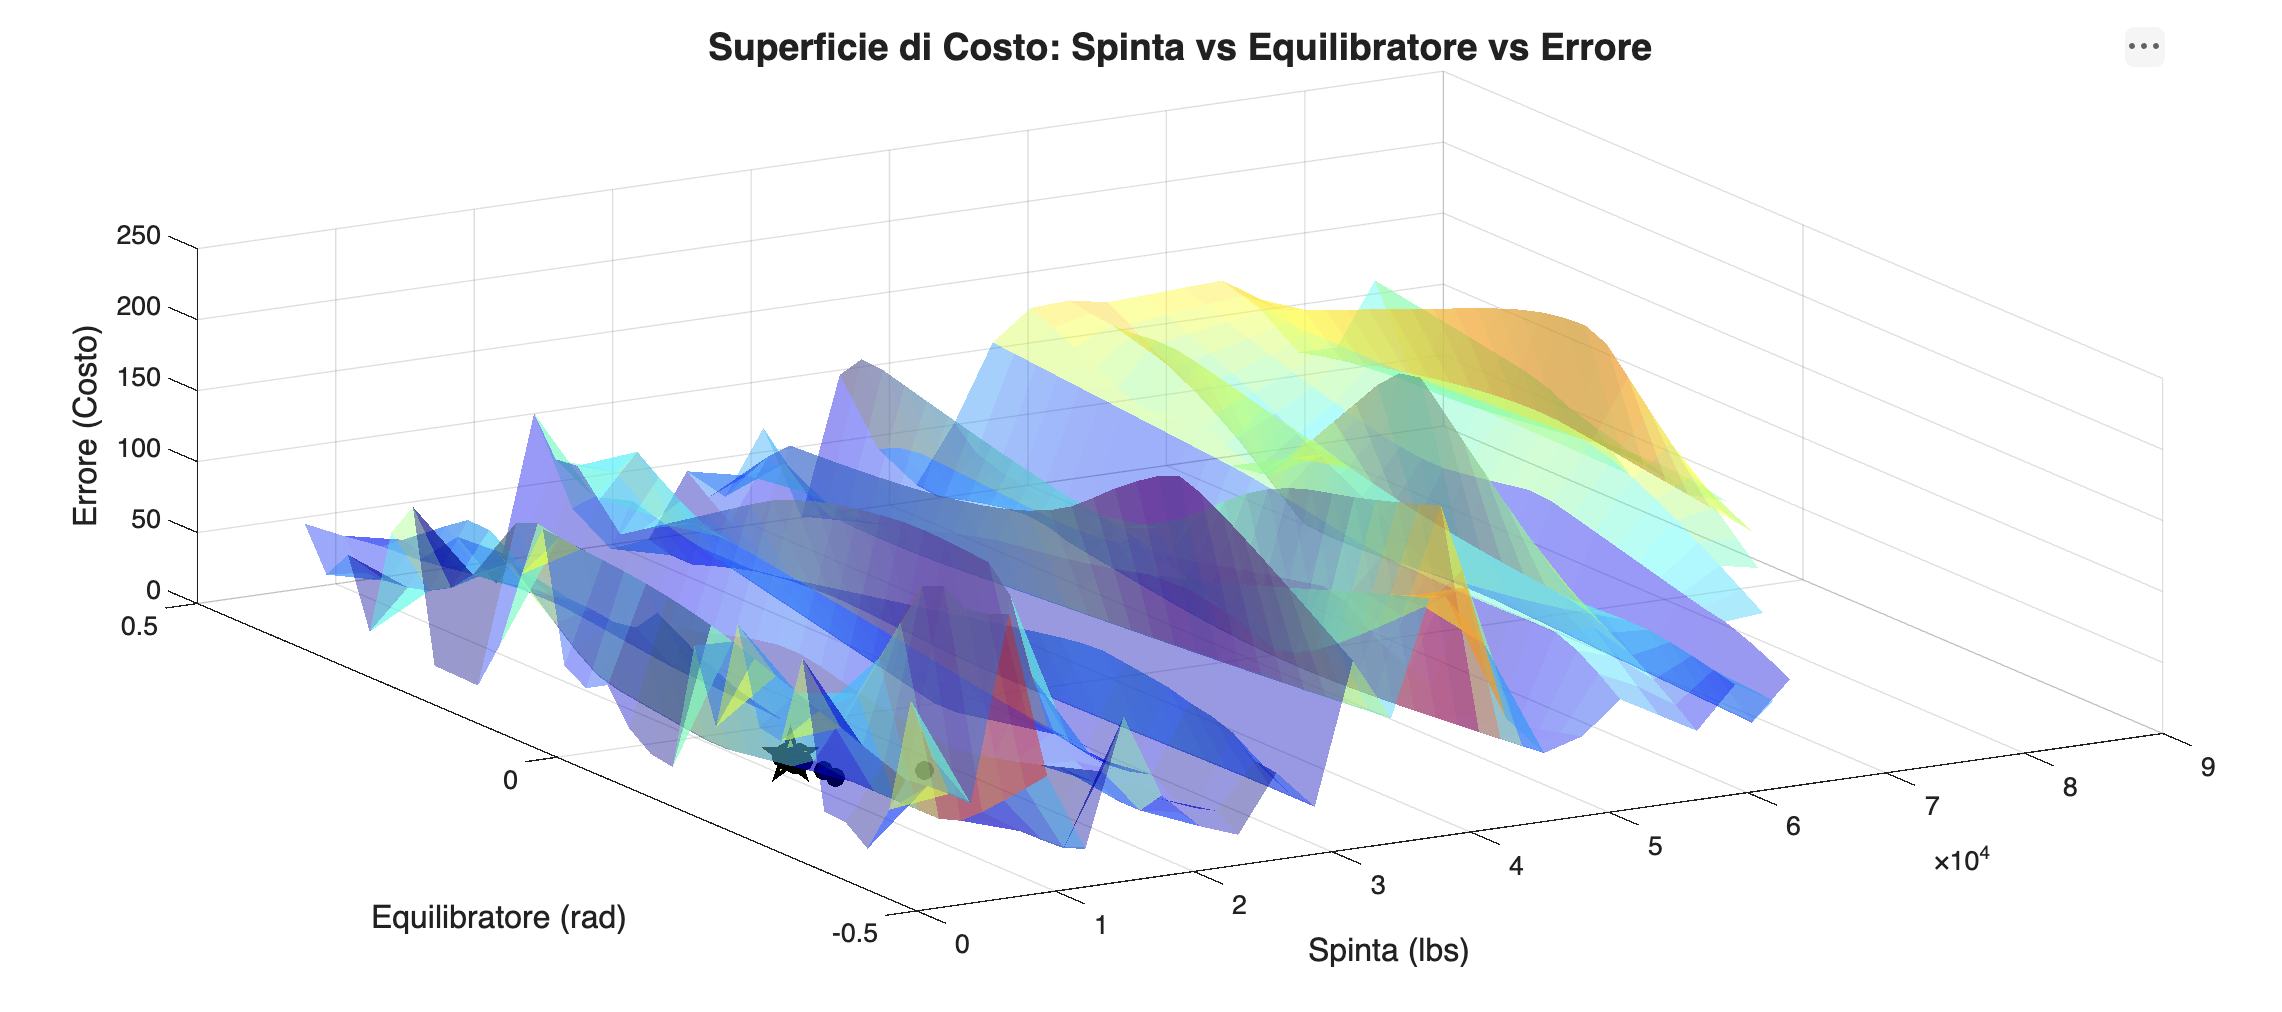
\includegraphics[width=1\textwidth]{Foto/AlgortimoPSO_.png}
	\caption{Algortimo PSO alla fine del suo funzionamento}
	\label{fig:PSO_fine}
\end{figure}


\begin{figure}[h!]
	\centering
	% Sostituisci 'punto_operativo.png' con il nome esatto del tuo screenshot caricato su Overleaf
	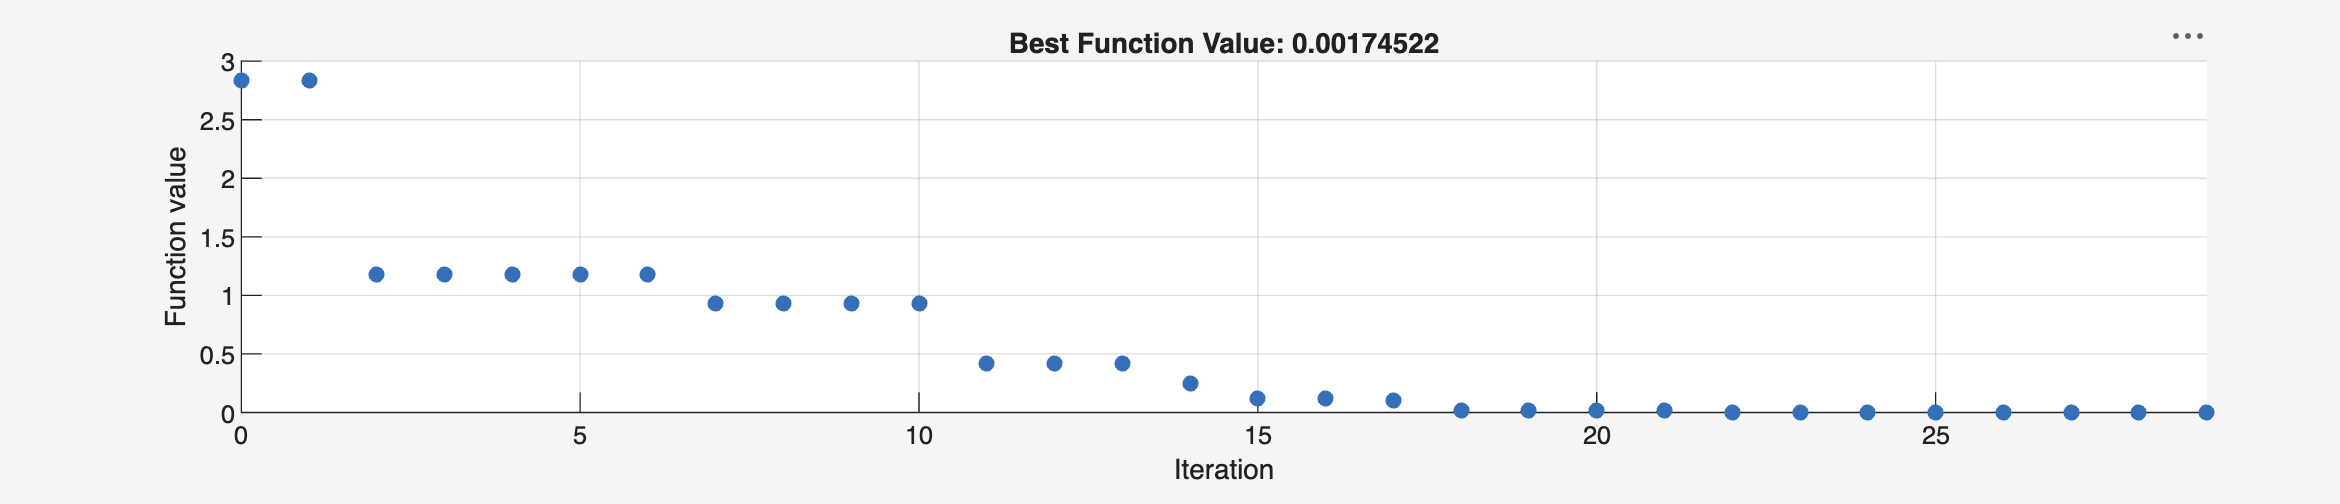
\includegraphics[width=1\textwidth]{Foto/funzionale_PSO.png}
	\caption{ Funzionale di costo dell'algoritmo}
	\label{fig:funzionale_costo_PSO}
\end{figure}
Questo algoritmo varia iterativamente gli angoli di assetto (come $\alpha$ e $\theta$) e i comandi (spinta ed equilibratore), esplorando lo spazio delle soluzioni in modo intelligente fino a minimizzare gli errori sulle derivate di stato. Il processo restituisce l'oggetto \textbf{\texttt{op}}, che contiene il punto di equilibrio esatto $(\mathbf{X}^*, \mathbf{U}^*)$, e l'oggetto \textbf{\texttt{opreport}}, che certifica l'avvenuta convergenza matematica mostrando residui tendenti a zero (garanzia di un vero equilibrio fisico in volo stazionario). I valori degli stati e degli ingressi di controllo calcolati a convergenza dall'algoritmo sono visualizzabili nella Figura \ref{fig:punto_operativo}.

\begin{figure}[h!]
    \centering
    % Sostituisci 'punto_operativo.png' con il nome esatto del tuo screenshot caricato su Overleaf
    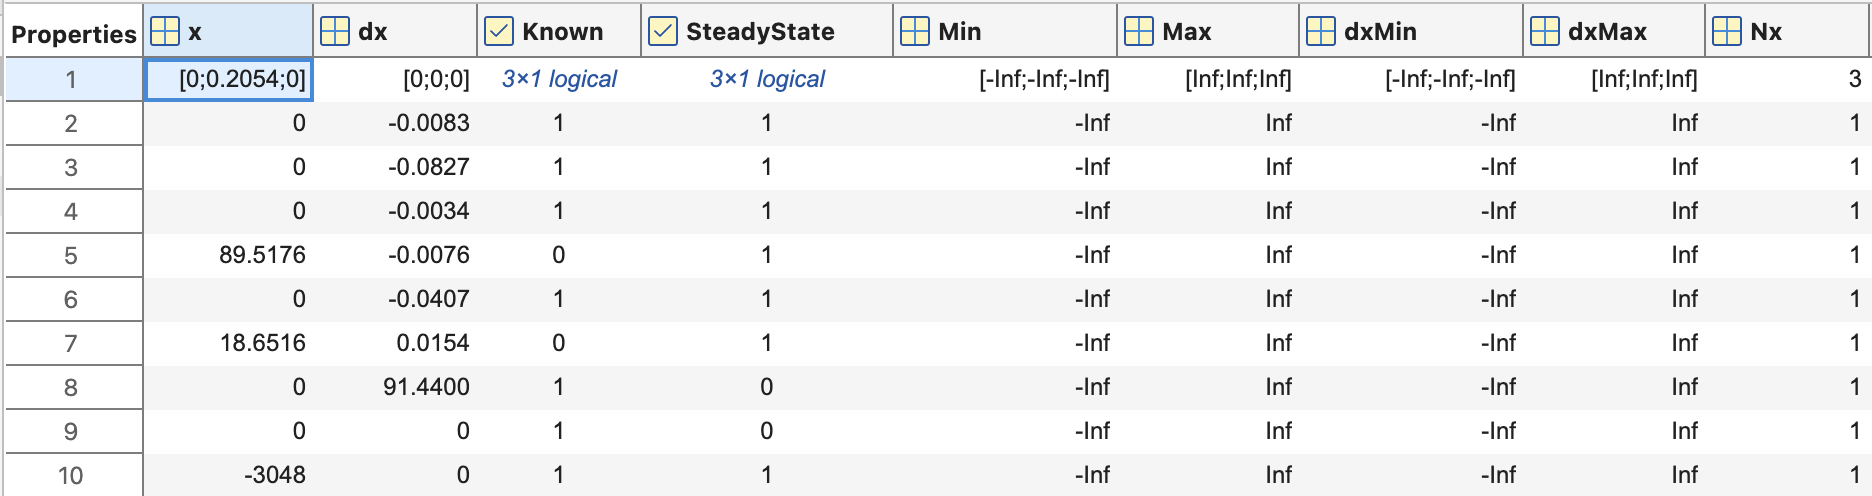
\includegraphics[width=1\textwidth]{Foto/OPREPORT.png}
    \caption{Report generato da MATLAB al termine dell'ottimizzazione, mostrante gli stati e gli ingressi di controllo del punto operativo (Trim) validato.}
    \label{fig:punto_operativo}
\end{figure}

\section{Linearizzazione dello spazio di stato}

Ottenuto il punto operativo \texttt{op}, si applica la teoria delle piccole perturbazioni. Definendo $\mathbf{x} = \mathbf{X} - \mathbf{X}^*$ e $\mathbf{u} = \mathbf{U} - \mathbf{U}^*$, si espande la funzione non lineare in serie di Taylor troncata al primo ordine, ottenendo il sistema lineare globale:
\begin{align}
\dot{\mathbf{x}}(t) &= A_{full} \mathbf{x}(t) + B_{full} \mathbf{u}(t) \\
\mathbf{y}(t) &= C_{full} \mathbf{x}(t) + D_{full} \mathbf{u}(t)
\end{align}

Tramite il comando \texttt{linearize}, l'algoritmo differenzia numericamente il modello restituendo le matrici Jacobiane complete $12 \times 12$. 
La matrice $A_{full} \in \mathbb{R}^{12 \times 12}$ mappa l'effetto che una perturbazione su ciascuno dei 12 stati ha sulle derivate (accelerazioni) di tutti gli altri 12 stati. Questa matrice contiene la dinamica \textit{completamente accoppiata} dell'F-16 in tutte le direzioni dello spazio.
\section{Analisi spettrale e autovalori}

Il comportamento in evoluzione libera del sistema perturbato è governato dall'equazione differenziale omogenea $\dot{\mathbf{x}}_{long} = A_{long} \mathbf{x}_{long}$. La stabilità di tale sistema dipende esclusivamente dalla matrice dinamica $A_{long}$ e viene analizzata calcolandone gli autovalori $\lambda$, ovvero le radici del polinomio caratteristico:
\begin{equation}
	\det(\lambda I - A_{long}) = 0
\end{equation}

Per il Teorema di Stabilità di Ljapunov applicato ai sistemi lineari:
\begin{itemize}
	\item Se tutti gli autovalori $\lambda_i = \sigma_i + j\omega_i$ possiedono parte reale strettamente negativa ($\sigma_i < 0$), il punto di equilibrio è \textbf{asintoticamente stabile}. Una perturbazione (es. una folata di vento) verrà smorzata nel tempo, riportando l'aereo in assetto.
	\item Se almeno un autovalore possiede parte reale positiva ($\sigma_i > 0$), il sistema è \textbf{instabile} e la perturbazione divergerà esponenzialmente.
\end{itemize}
Eseguendo il calcolo degli autovalori sulla realizzazione minima del sistema longitudinale (tramite il comando \texttt{pole(sys\_long\_min)}), i risultati estratti da MATLAB rivelano la vera natura aerodinamica dell'F-16. A differenza degli aerei civili convenzionali — che presentano tipicamente due coppie di autovalori complessi coniugati stabili (identificativi dei classici modi di Fugoide e Corto Periodo utili per studiare la dinamica veloce e lenta del controllo longitudinale), l'F-16 è progettato con \textit{stabilità statica rilassata} per massimizzare l'agilità in combattimento. L'analisi numerica restituisce infatti quattro autovalori: \textbf{tre con parte reale strettamente negativa e uno con parte reale positiva}. Questo singolo polo posizionato nel semipiano destro ($s > 0$) genera un modo aperiodico divergente. Ciò dimostra matematicamente che la dinamica longitudinale dell'F-16 ad anello aperto è \textbf{intrinsecamente instabile}. Qualsiasi perturbazione esterna, per quanto infinitesima, provocherebbe un rapido e incontrollabile ribaltamento del muso. Di conseguenza, risulta fisicamente impossibile pilotare il velivolo in sicurezza senza un'assistenza elettronica, rendendo categoricamente obbligatoria la sintesi di un sistema di controllo attivo FCS(Flight Control System) in retroazione per stabilizzare il plant. Il computer di bordo e la sua realizzazione real-time si trova a questo capitolo \ref{sec:fly-by-wire}.
La distribuzione spaziale degli autovalori è confermata e visualizzabile graficamente tramite la mappa poli-zeri del sistema, generata dal comando \texttt{pzmap} e riportata in Figura \ref{fig:pzmap_long}. Nel grafico è immediatamente identificabile la radice instabile ("X") posta a destra dell'asse immaginario.

\begin{figure}[h!]
	\centering
	% Sostituisci 'nome_tua_immagine.png' con il file generato da MATLAB
	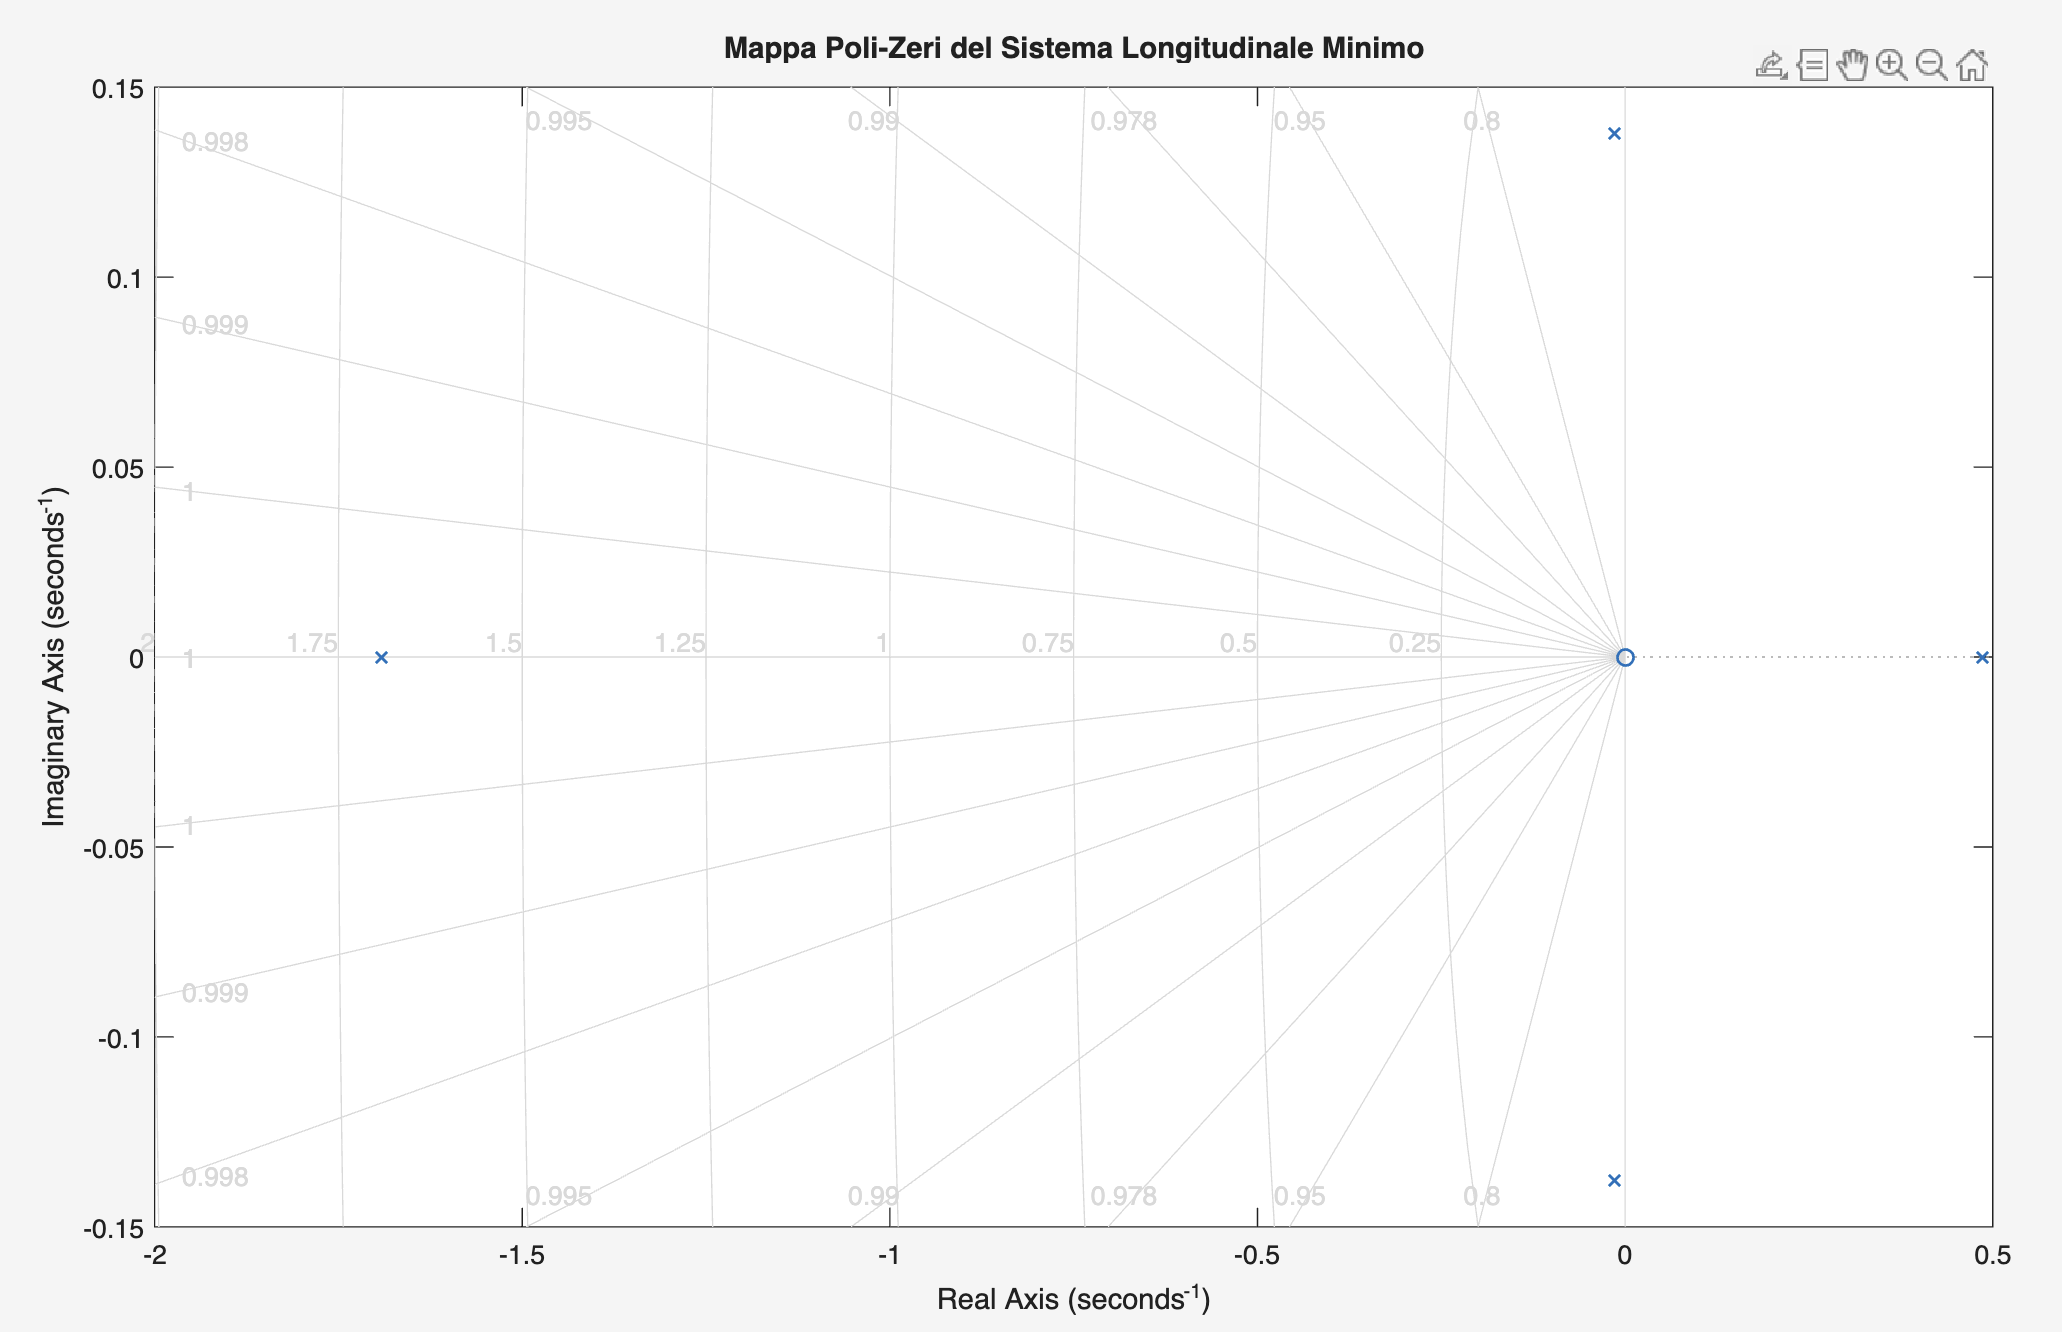
\includegraphics[width=0.9\textwidth]{Foto/PZGraph.png}
	\caption{Mappa Poli-Zeri (pzmap) della realizzazione minima longitudinale. Evidenza del polo instabile a parte reale positiva.}
	\label{fig:pzmap_long}
\end{figure}

\section{Disaccoppiamento delle dinamiche}
\label{sec:cap8_3}
Si procede quindi all'estrazione (partizionamento) del \textbf{Sottosistema Longitudinale}. Osservando la convenzione del vettore di stato dell'F-16 di Stevens e Lewis, \cite{stevens2015aircraft}: Per isolare la dinamica longitudinale dal modello aerodinamico completo a 6 gradi di libertà, le matrici di stato vengono estratte selezionando opportunamente gli indici associati alle variabili di interesse. L'operazione di partizionamento permette di ottenere il sottosistema ridotto come segue:

\begin{equation}
	\begin{aligned}
		A_{long} &= A_{\text{full}}(ix, ix) \\
		B _{long}&= B_{\text{full}}(ix, iu) \\
		C_{long}&= C_{\text{full}}(iy, ix) \\
		D_{long} &= D_{\text{full}}(iy, iu)
	\end{aligned}
\end{equation}

Dove i vettori degli indici $ix$, $iu$ e $iy$ definiscono rispettivamente gli stati, gli ingressi e le uscite del modello longitudinale estratti dal simulatore:

\textbf{Vettore degli Stati ($ix = [2, 5, 7, 9]$):}
\begin{itemize}
	\item $\theta$ (Pitch angle) $\rightarrow$ Indice \textbf{2}
	\item $q$ (Pitch rate) $\rightarrow$ Indice \textbf{5}
	\item $U$ (Body X-axis velocity) $\rightarrow$ Indice \textbf{7}
	\item $W$ (Body Z-axis velocity) $\rightarrow$ Indice \textbf{9}
	\begin{itemize}
		\item[$\circ$] {\small \textit{Nota: $U$ e $W$ sono le componenti della velocità sugli assi corpo. Da queste si ricavano le variabili aerodinamiche per il controllo di volo, ovvero la velocità totale $V_t = \sqrt{U^2 + W^2}$ e l'angolo d'attacco $\alpha = \arctan(W/U)$.}}
	\end{itemize}
\end{itemize}

\vspace{0.3cm}

\textbf{Vettore degli Ingressi ($iu = [1, 2, 5, 6, 8]$):}
\begin{itemize}
	\item \texttt{Thrust} (Manetta) $\rightarrow$ Indice \textbf{1}
	\item \texttt{F16/ele} (Equilibratore / Elevator) $\rightarrow$ Indice \textbf{2}
	\item \texttt{F16/lef} (Flap al Bordo d'Attacco / LEF) $\rightarrow$ Indice \textbf{5}
	\item \texttt{F16 gust1} (Disturbo: Raffica di vento asse X) $\rightarrow$ Indice \textbf{6}
	\item \texttt{F16 Gust3} (Disturbo: Raffica di vento asse Z) $\rightarrow$ Indice \textbf{8}
\end{itemize}

\vspace{0.3cm}

\textbf{Vettore delle Uscite ($iy = [7, 8, 13, 15, 17, 19]$):}
\begin{itemize}
	\item $V_t$ (True Airspeed) $\rightarrow$ Indice \textbf{7}
	\item $\alpha$ (Angle of Attack) $\rightarrow$ Indice \textbf{8}
	\item $\gamma$ (Flight Path Angle) $\rightarrow$ Indice \textbf{13}
	\item $q$ (Pitch rate in uscita) $\rightarrow$ Indice \textbf{15}
	\item $a_x$ (Accelerazione asse X / xbdd) $\rightarrow$ Indice \textbf{17}
	\item $a_z$ (Accelerazione asse Z / zbdd) $\rightarrow$ Indice \textbf{19}
\end{itemize}
Di conseguenza, il vettore di estrazione degli stati è rigorosamente \texttt{ix = [2, 5, 7, 9]}. Allo stesso modo, tramite il vettore \texttt{iu}, si isolano i comandi che agiscono in modo simmetrico (Spinta, Equilibratore, Flap) e le raffiche di vento, escludendo alettoni e timone; mentre con \texttt{iy} si selezionano le sole variabili di output utili al controllo longitudinale. 

L'estrazione in MATLAB avviene applicando questi vettori come veri e propri "filtri matematici" sull'impianto completo:

\begin{itemize}
    \item \textbf{Matrice Dinamica ($A$):} Il comando \texttt{A\_long = A\_full(ix, ix)} estrae la sottomatrice $A_{long} \in \mathbb{R}^{4 \times 4}$. Questa descrive esclusivamente come beccheggio, rateo, e le velocità sull'asse corpo interagiscano tra loro, isolando il nucleo puro della dinamica longitudinale transitoria.
    \item \textbf{Matrice degli Ingressi ($\mathbf{B}_{long}$ e sua scomposizione):} Il partizionamento \texttt{B\_long = B\_full(ix, iu)} genera inizialmente la sottomatrice $\mathbf{B}_{long} \in \mathbb{R}^{4 \times 5}$. Essa mappa l'efficacia aerodinamica e propulsiva dei comandi longitudinali (e l'impatto dei disturbi del vento) direttamente sulle derivate degli stati, scartando qualsiasi accoppiamento "sporco" con la dinamica latero-direzionale. 
    
    Tuttavia, ai fini della sintesi delle leggi di controllo, lo script procede con una fondamentale scomposizione algoritmica di tale matrice:
    \begin{equation}
    	\mathbf{B}_{long} = \big[ \mathbf{B}_{ctrl} \;\big|\; \mathbf{B}_{wind} \big]
    \end{equation}
    
    Questa operazione divide la matrice originaria in due sottomatrici distinte: $\mathbf{B}_{ctrl}$ isola esclusivamente le colonne relative agli attuatori fisicamente comandabili dal \textit{Flight Control Computer} (manetta $\delta_{th}$, elevatore $\delta_e$ e flap di bordo d'attacco $\delta_{lef}$), mentre $\mathbf{B}_{wind}$ raggruppa le colonne relative agli ingressi di disturbo atmosferico non controllabili. Come anticipato nel \ref{cap:5},e approfondito nel \ref{sec:Capitolo 12Wind}, questa separazione è il presupposto matematico obbligatorio affinché l'algoritmo di controllo agisca unicamente sui comandi fisici del velivolo per reiezione dei disturbi, senza tentare matematicamente di "comandare il vento".

    \item \textbf{Matrice di Uscita ($C$):} L'estrazione \texttt{C\_long = C\_full(iy, ix)} produce la matrice $C_{long} \in \mathbb{R}^{6 \times 4}$. Questa matrice definisce il legame algebrico e cinematico che trasforma gli stati interni del corpo rigido nelle grandezze fisiche misurate dai sensori (come la velocità totale $V_t$, l'incidenza $\alpha$ e il rateo di beccheggio in uscita).

    \item \textbf{Matrice di Trasmissione Diretta ($D$):} Infine, \texttt{D\_long = D\_full(iy, iu)} fornisce la matrice di feedthrough $D_{long} \in \mathbb{R}^{6 \times 5}$. La corretta estrazione di questa matrice è vitale per la fedeltà del modello, poiché modella gli effetti istantanei: cattura, ad esempio, come una rapida deflessione dell'equilibratore generi un picco immediato di accelerazione verticale ($a_z$) prima ancora che il velivolo abbia fisicamente il tempo di ruotare.
\end{itemize}


\section{Rappresentazione MIMO e funzioni di trasferimento}
Il modello linearizzato nello Spazio degli Stati fornisce una descrizione completa della dinamica interna del velivolo. Tuttavia, per l'analisi nel dominio della frequenza e la progettazione dei classici controllori (come il PID per il mantenimento della quota o del beccheggio), è necessario mappare la relazione diretta tra gli ingressi di controllo (cause) e le uscite misurate (effetti).

Essendo l'F-16 un sistema \textbf{MIMO} (\textit{Multiple-Input Multiple-Output}), non è descrivibile da una singola funzione di trasferimento, ma richiede una \textbf{Matrice delle Funzioni di Trasferimento}, indicata con $G(s)$.

\subsection{Derivazione Matematica}
Si consideri il sistema lineare tempo-invariante (LTI) precedentemente estratto:
\begin{align}
\dot{\mathbf{x}}(t) &= A \mathbf{x}(t) + B \mathbf{u}(t) \\
\mathbf{y}(t) &= C \mathbf{x}(t) + D \mathbf{u}(t)
\end{align}
Applicando la Trasformata di Laplace ad ambo i membri e assumendo condizioni iniziali nulle ($\mathbf{x}(0) = \mathbf{0}$), l'equazione di stato diviene:
\begin{equation}
s\mathbf{X}(s) = A \mathbf{X}(s) + B \mathbf{U}(s) \implies \mathbf{X}(s) = (sI - A)^{-1} B \mathbf{U}(s)
\end{equation}
Sostituendo $\mathbf{X}(s)$ nell'equazione di uscita, si ottiene la relazione ingresso-uscita nel dominio di Laplace:
\begin{equation}
\mathbf{Y}(s) = \left[ C(sI - A)^{-1} B + D \right] \mathbf{U}(s)
\end{equation}
La matrice $G(s) = C(sI - A)^{-1} B + D$ è la Matrice delle Funzioni di Trasferimento. Se il vettore degli ingressi $\mathbf{U}$ ha dimensione $m$ e il vettore delle uscite $\mathbf{Y}$ ha dimensione $p$, $G(s)$ sarà una matrice di dimensione $p \times m$. 

Ogni singolo elemento $G_{i,j}(s)$ della matrice è una funzione di trasferimento SISO (\textit{Single-Input Single-Output}) costituita dal rapporto tra due polinomi complessi, e descrive come il $j$-esimo ingresso influenzi l'$i$-esima uscita:
\begin{equation}
G_{i,j}(s) = \frac{Y_i(s)}{U_j(s)}
\end{equation}

% ==========================================
% CAPITOLO 9: REALIZZAZIONE MINIMA E ANALISI MIMO DA RIVEDERE
% ==========================================
